\subsection{Perturbation of motion in a constant field}

We first reason heuristically to see that this idea is valid. Comparing the trajectories for $b=0.01$ and $ 0.001$ in \cref{subfig:weakcomparisonA} and \ref{subfig:weakcomparisonB}, we see that the radius of the trajectory is $\approx250$ and $\approx2500$, respectively. If we assume this is the value of the Larmor radius $\hat L$ in each case, then we see $\hat L\varpropto 1/b$ or $\hat b\varpropto b$. Now, comparing the trajectories for $b=0.01$ in \cref{subfig:weakcomparisonA} and \ref{subfig:weakcomparisonC}, we see halving the radius $R$ of the magnetic bumps roughly quadruples the radius $\hat L$ from 250 to 1000, that is, $\hat L\varpropto 1/R^2$, and the strength then relates as $\hat b \varpropto R^2b$. The task then is to determine $C\in\mathbb R$ such that $\hat b = CR^2b$.

We can reason another way. Focusing on $[0,1]^2$, we would like the uniform field $\mathbf{\hat B}=\nabla\times \hat A=(-\hat bq_2,0,0)$ to deflect trajectories as would $\mathbf B =\nabla\times A$. How much a trajectory is deflected depends on the flux of the field, since the flux measures the ``flow'' of the field through a surface. Equating the fluxes $\Phi_{\mathbf B}=\Phi_{\mathbf{\hat B}}$, we can compute the required strength $\hat b$ for $\hat B$. The flux of $\mathbf B$ through a bounded region in the plane is given by:
\begin{align*}
\Phi_{\mathbf B} 
  = \iint_{S}\mathbf B\cdot dA
  = \iint_{S}\nabla\times A\cdot dA
  = \iint_{S}(0,0,b)\cdot (0,0,1) dA = b A(S), 
\end{align*}
where $A(S)$ denotes the area of the surface. In our case, $\Phi_{\mathbf{\hat B}}=\Phi_{\mathbf B}$ implies $\hat b = \pi R^2 b$, which is about what we expected. Now, we should numerically test this hypothesis. To test the validity of the relation, we give two tests, the results of which can be found in \cref{fig:modeling}. The first test:
\begin{enumerate}
\item For $1\le i\le 50$, sample $(R_i, b_i)$ uniformly from $[0.25,0.45]\times[10^{-10},10^{-6}]$ 
\item For $R_i, b_i$ uniformly sample initial conditions $X_{ij},V_{ij}$ with $1\le j\le 20$.
\item Using the method in \cite{Coope93}, fit a circle to the trajectory of each $X_{ij}, V_{ij}$, the radius of which is $\hat L_{ij}$. We take the average $\hat L_i=\sum_{j=1}^{20}\hat L_{ij}/20$. 
\item Via a least squares method, we fit a general cubic:
\begin{align*}
a_0 + a_1R_i + &a_2b_i + a_3R_i^2 \\
  &+ a_4R_ib_i + a_5b_i^2 + a_6R_i^3 +a_7R_i^2b_i+a_8R_ib_i^2+a_9b_i^3=1/\hat L_i.
\end{align*}
\end{enumerate}
The second test is similar, we fix $R_i=1/3$, and fit a line $a_0+a_1R_i^2b_i=1/\hat L_i$. We opt to fit a general cubic function to avoid any bias in reasoning. We should expect after fitting that only $a_7$ contributes significantly.

 


The coefficients of the fitted cubic surface in \cref{subfig:3dfitting} come out to
\begin{align*}
a_0&\approx  6.7\cdot10^{-8},	&
a_1&\approx -6.2\cdot10^{-7},	&
a_2&\approx  6.7\cdot10^{-3},\\
a_3&\approx  1.9\cdot10^{-6},	&
a_4&\approx -5.3\cdot10^{-2},	&
a_5&\approx -1.9\cdot10^{+2},\\
a_6&\approx -1.8\cdot10^{-6},	&
a_7&\approx  3.2,				&
a_8&\approx  -6.6\cdot10^{+1},\\
a_9&\approx  -3.0\cdot10^{-4},
\end{align*} 
the values of $a_0$ to $a_4$, $a_6$ and $a_9$ are negligible as expected, likewise $a_7\approx\pi$. We notice that $a_5$ and $a_8$ are quite large but we reason that the contribution of their respective monomial term is still small, since both contain a factor of $b^2$ which has an order of magnitude at most $10^{-6}$. The coefficients of the fitted line in \cref{subfig:2dfitting} are $a_0\approx 4.4\cdot10^{-10}$ and $a_1\approx3.12$, which can be explained in the same way. So, the relation $\hat b =\pi R^2b$ seems valid, and this motivates perturbing a uniform magnetic field into the bump field.

\begin{figure}[!ht]
\centering
\begin{subfigure}[!th]{0.49\textwidth}
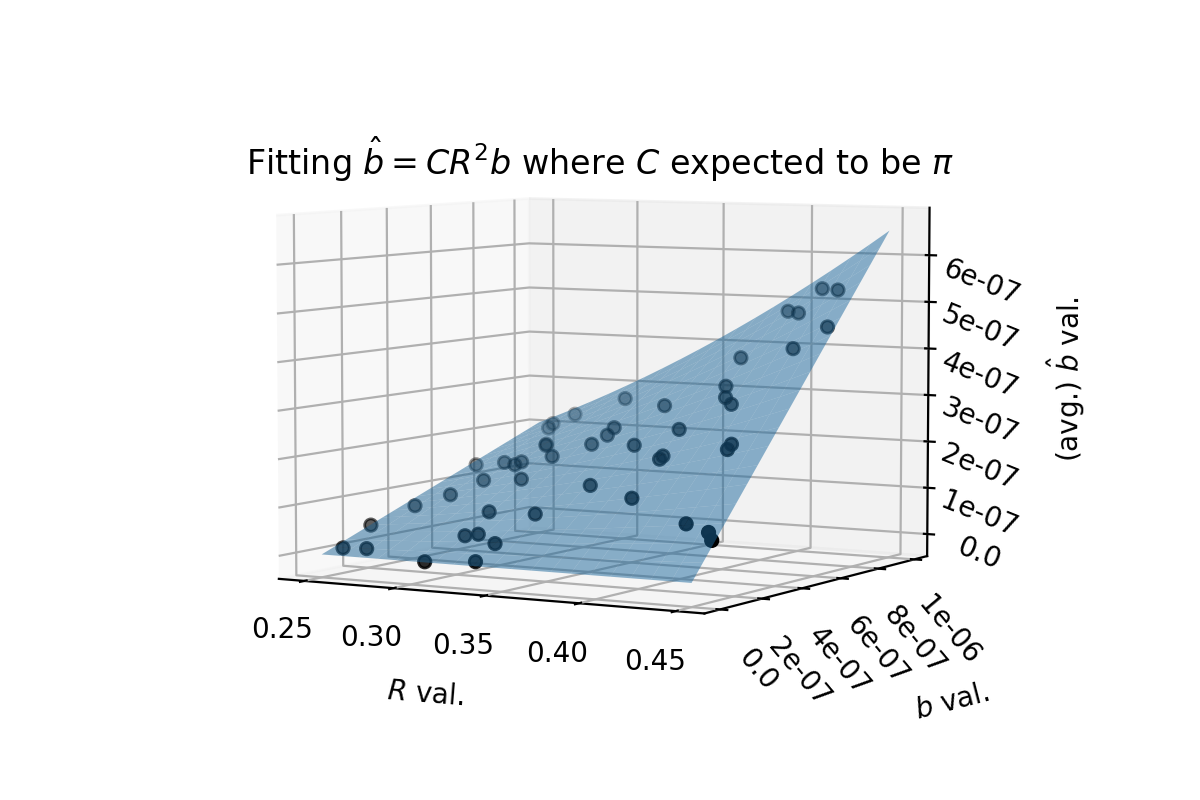
\includegraphics[width=\textwidth, trim={3cm 1cm 1cm 1.5cm}, clip]{kam_approx_surface.png}
\caption{Fitting a cubic surface}
\label{subfig:3dfitting}
\end{subfigure}
%
\begin{subfigure}[!th]{0.49\textwidth}
\centering
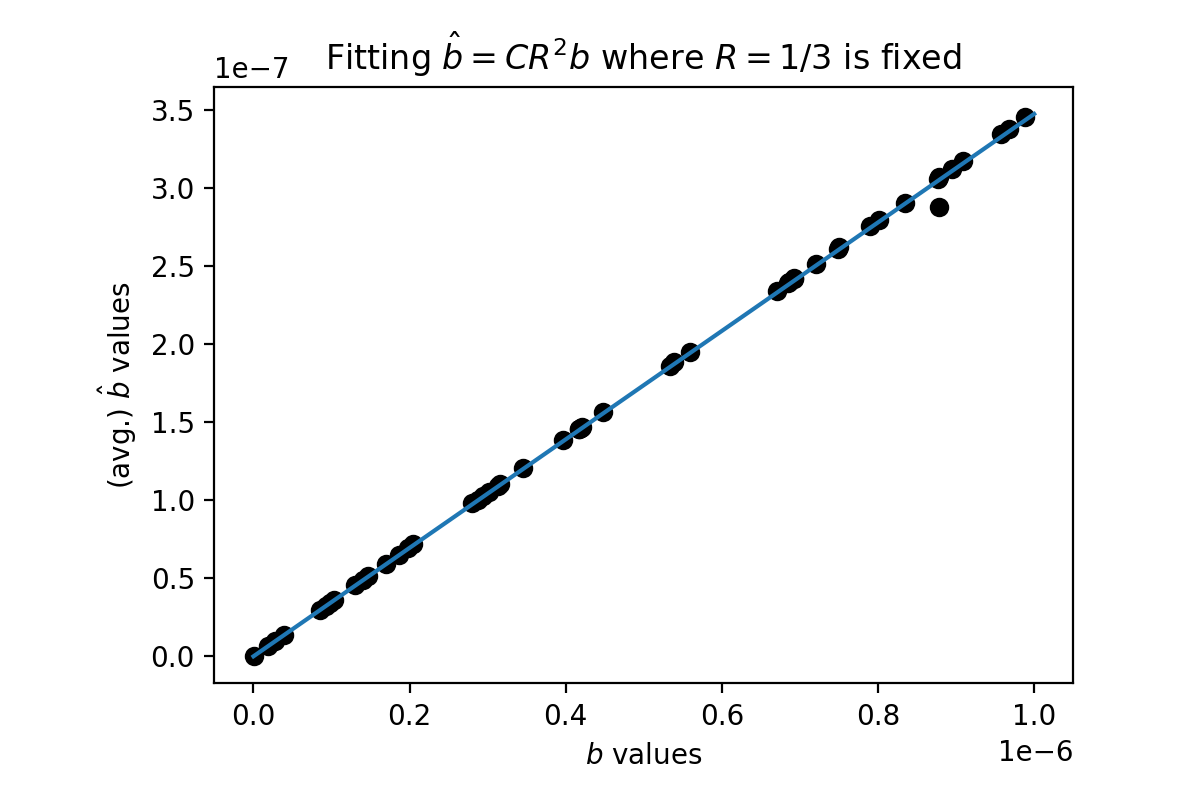
\includegraphics[width=\textwidth, trim={1.25cm 0.25cm 1.5cm 0.5cm}, clip]{kam_approx_line.png}
\caption{Fitting a line}
\label{subfig:2dfitting}
\end{subfigure}
\caption{Plots of data and fitted polynomial models.}
\label{fig:modeling}
\end{figure}


Overall, the results show that our assumptions are plausible, we approximately see $\pi$ in the coefficient. The results are not as precise as desired but that can be due to randomly choosing the initial conditions for the trajectories. The circular trajectories correspond to invariant tori, and since not all tori are preserved under the perturbation, we expect that, chosen at random, some trajectories will not follow closely a circular path. Similarly, the chosen range for sampling $R$ and $b$ could be too large, though in tests we made that we omit here, we noticed that the relation holds more or less for a wider range of $[0.1, 0.45]\times[10^{-16}, 10^{-2}]$. 

